\section{Hierarchical Deterministic Wallets(BIP32,BIP44)}

出于隐私性的考虑,中本聪在比特币的白皮书中建议:\textbf{A new key pair should be used 
for each transaction to keep them from being linked to a common owner.} 
为了防止每次交易后都需要对新生成的公私钥进行备份,钱包客户端需要维护一个预留的密钥池。
这种方式给用户在不同客户端之间进行切换、以及钱包对用户私钥的管理带来了困难:在切换时,用户需要导出/导入所有相关地址的私钥,并且不能在不同的系统上同时使用钱包。
分层确定性钱包从根节点确定性派生密钥树的方法很好地解决了这个问题。

分层确定性(HD)钱包是由Pieter Wuille在2012年于BIP32中提出的,在该协议下,
钱包从根节点出发,按照层级结构以一种确定性的方式从parent key 派生 child key,
从而建立起一棵由根节点完全派生的树。因此,当用户在两个支持该协议的不同客户端之间进行切换时,密钥的导入、
导出只需要复制根节点(主密钥)的信息,钱包可以根据根节点和该协议规定的派生方法确定性地派生出整棵密钥树。
因此,用户可以方便地在不同客户端之间切换,钱包也可以依据密钥的派生层级对密钥进行逻辑上的分层管理。
  
此外,该协议允许child private/public key的派生过程相互独立,
即parent private key 可以派生出 child private/public key,
而parent public key只能派生出 child public key。
它保证了在不安全的环境中,在没有parent private key 访问权限的情况下也
可以进行child public key的派生,防止父私钥的泄露。
同时,钱包的树状结构有助于用户对访问权限进行选择性的共享(这取决于共享的密钥所处的层级,
以及共享的是私钥还是公钥)。  

由于BIP32\footnote{https://github.com/bitcoin/bips/blob/
33e040b7bdf5d937599d2401454878d6293476c9/bip-0032.mediawiki}着重讲述分层确定性钱包的原理,
对于客户端如何实现并没有做严格的限制,
因此,2014年,Marek Palatinus和Pavol Rusnak 
提出了BIP44\footnote{https://github.com/bitcoin/bips/blob/master/bip-0044.mediawiki},
在BIP32的基础上对钱包具体的实现方式、 不同层级的逻辑含义进行了规定。目前已经支持BIP44的钱包有
Mycelium Bitcoin Wallet,Copay, CoinVault,Samourai,Coinomi,Trezor,Keepkey,Ledger Wallet,
21 Machine Wallet, Trust Wallet。  

\subsection{密钥派生}

\textbf{扩展密钥}

 在使用该协议从父节点派生子节点时,实际上使用的是512比特的扩展密钥$(k,c)/(K,c)$,
 其中$k$代表私钥,$K$代表公钥,$c$则称为chain code,作为额外的256比特的熵。
 对于扩展公私钥对,其中只有公私钥部分不同,chain code是相同的。
 
 每一个扩展密钥都有最多$2^{31}$个 normal child key和$2^{31}$个hardened child key, 
 normal child key对应的index从0到$2^{31}-1$,hardened child key的index 
 则从$2^{31}$ 到$2^{32}-1$,为便于表示,对于hardened key的index,$i+2^{31}$记为 $i_H$。Hardened node引入的目的是为了增强整个方案的安全性,具体原理在Security\ref{sec-security}一节会详细介绍。
 下面首先介绍从父节点到子节点的密钥派生过程。

\subsubsection{Private Parent Key $\rightarrow$ Private Child Key}
 
\begin{algorithm}[tbp]\footnotesize
\caption{Private Child Key Derivation}
  	\begin{algorithmic}[1]
	    \STATE The function $CKDpriv((k_{par}, c_{par}), i) \rightarrow (k
		_i, c_i)$ computes a child extended private key from the 
		parent extended private key:
		\STATE Check whether $i \geq 2^{31}$ (whether the child is a hardened key).  
		\IF {hardened child}
			\STATE let I = HMAC-SHA512($Key = c_{par}$, Data = 0x00 || 
			$ser_{256}(k_{par}$) || $ser_{32}$(i)). (Note: The 0x00 pads 
			the private key to make it 33 bytes long.)  
		\ELSE
			\STATE let I = HMAC-SHA512(Key = $c_{par}$, 
			Data = $ser_P$(point($k_{par}$)) || $ser_{32}$(i)).  
		\ENDIF
		\STATE Split I into two 32-byte sequences, $I_L$ and $I_R$.
		\STATE The returned child key $k_i$ is $parse_{256}(I_L)$ + $k_{par}$ (mod n).
		\STATE The returned chain code $c_i$ is $I_R$.  
		\STATE In case parse256($I_L) \geq n$ or $k_i = 0$, the resulting key is invalid, 
		and one should proceed with the next value for i. 
		(Note: this has probability lower than 1 in $2^{127}$.)  
    \end{algorithmic}
\end{algorithm}

需要注意的是,对于hardened child node和normal child node的派生方法是有区别的:
在派生private normal child key 时,首先使用父节点的私钥计算出对应的公钥后(即$point(k_{par}$)),
将公钥与child的index `i` 级联后作为data,父节点的chain code作为key,一起送入HMAC-SHA512进行运算。
而hardened child node 则使用0x00 || $ser_{256}(k_{par}$) || $ser_{32}$(i)作为HMAC-SHA512的data,
这也就导致了hardened child 只能由private parent key来派生(无论是计算child private key还是public child key)。

\begin{figure}[h]
\centering
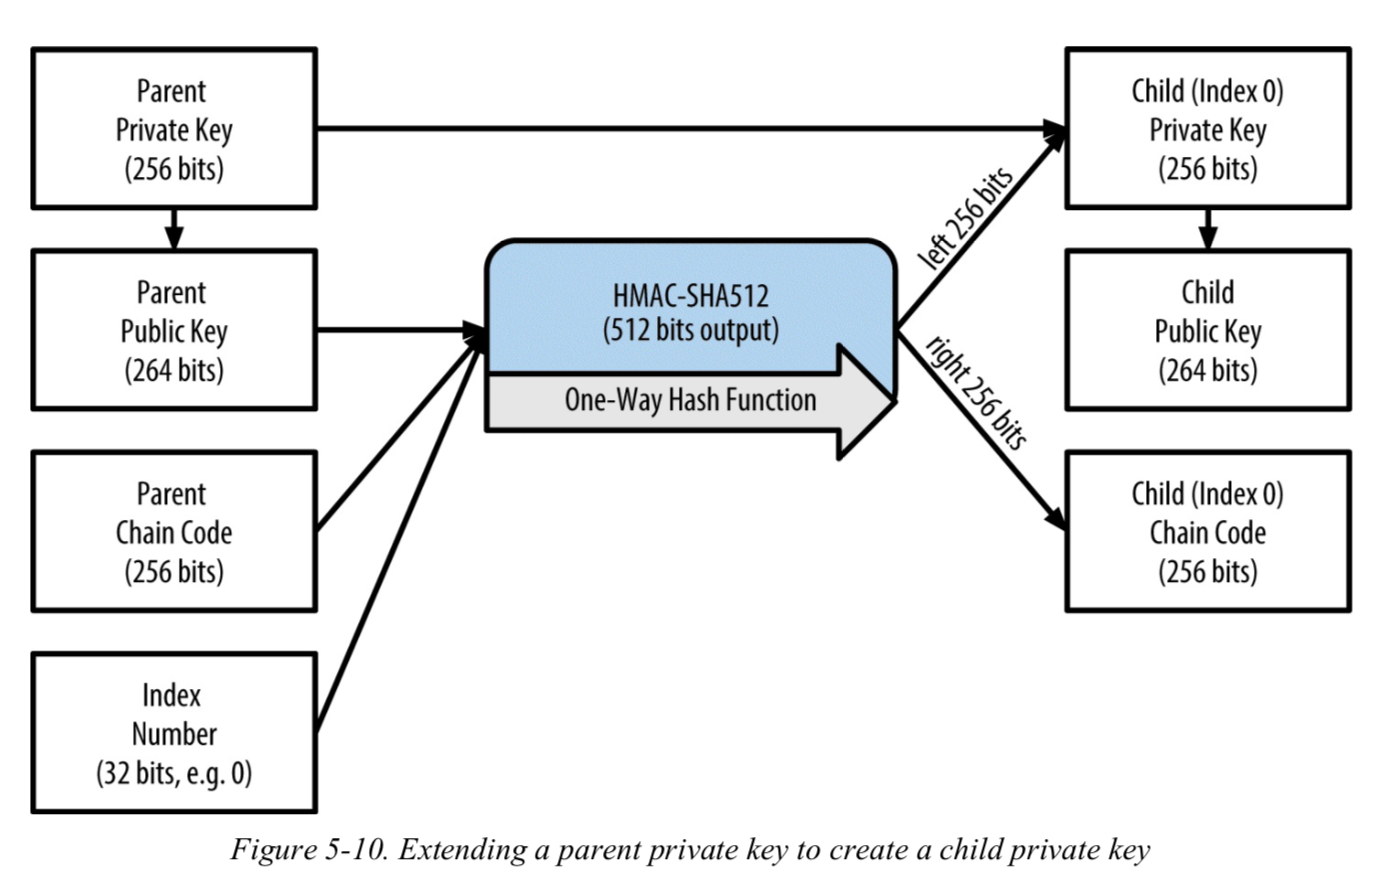
\includegraphics[width=.7\textwidth]{./CKDpriv.png}
\caption{Normal child 的派生过程(图片来自《Master Bitcoin》)}\label{fig-parsesig}
\end{figure}


\begin{figure}[h]
\centering
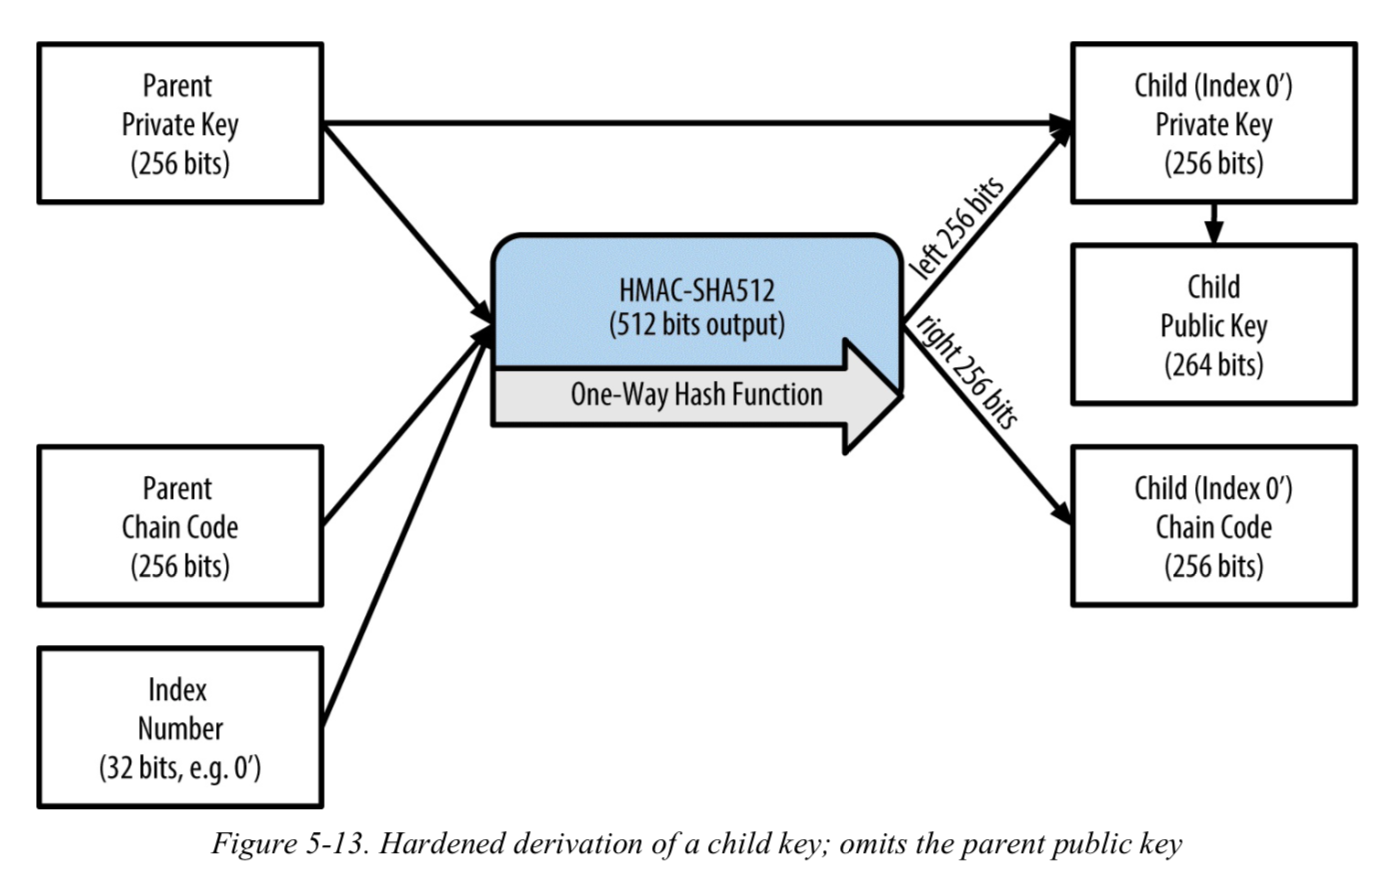
\includegraphics[width=.7\textwidth]{./CKDpriv2.png}
\caption{Hardened child 的派生过程(图片来自《Master Bitcoin》)}\label{fig-parsesig}
\end{figure}



\subsubsection{Public Parent Key $\rightarrow$ Public Child Key}

\begin{figure}[h]
\centering
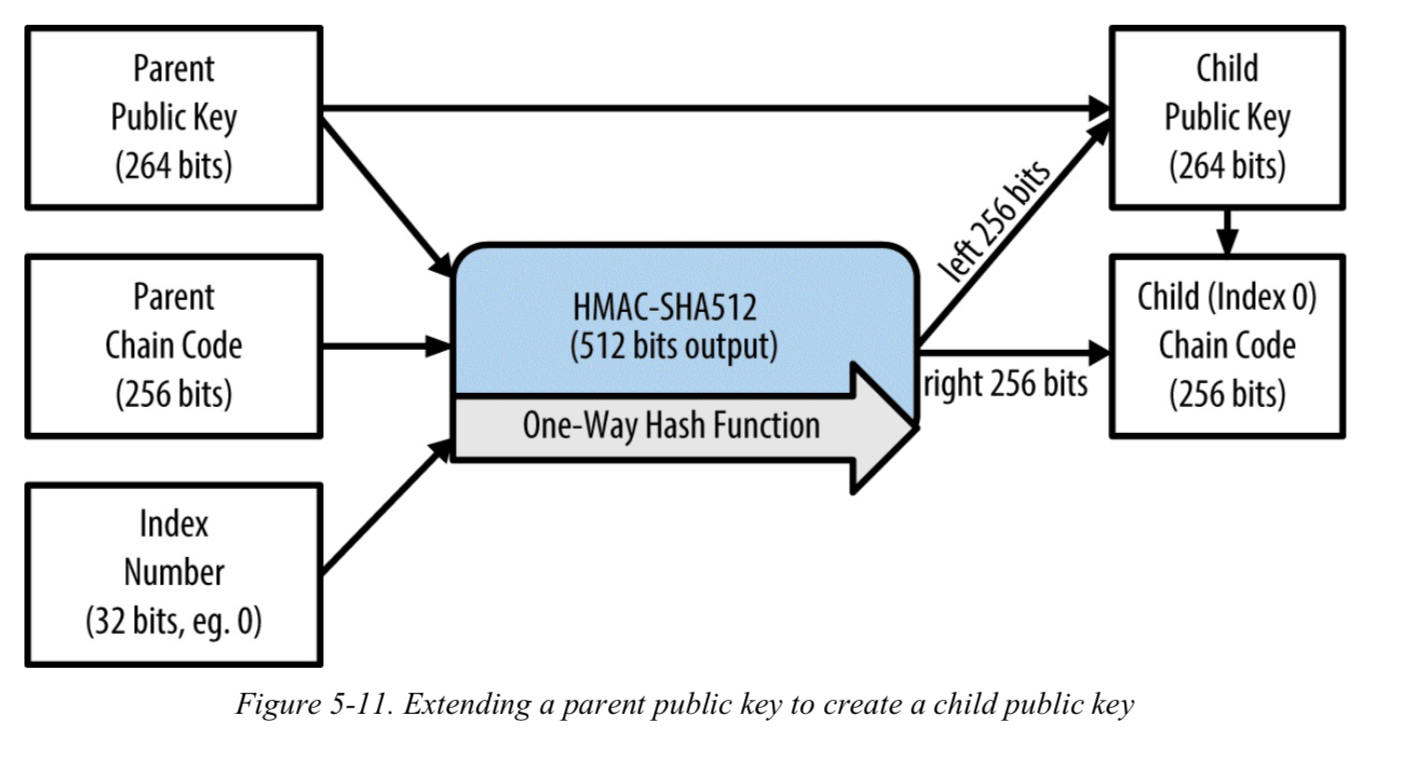
\includegraphics[width=.7\textwidth]{./CKDpub.png}
\caption{}\label{fig-parsesig}
\end{figure}

\begin{algorithm}[tbp]\footnotesize
\caption{Public Child Key Derivation}
  	\begin{algorithmic}[1]
	    \STATE The function $CKDpub((K_{par}, c_{par}), i) \rightarrow (K_i, c_i)$ computes 
	    a child extended public key from the parent extended public key. 
	    It is only defined for non-hardened child keys.
		\STATE Check whether $i \geq 2^{31}$ (whether the child is a hardened key).
		\IF {hardened child}
			\STATE return failure  
		\ELSE
			\STATE let I = HMAC-SHA512($Key = c_{par}, Data = ser_P(K_{par})$ || $ser_{32}(i)$). 
		\ENDIF
		\STATE Split I into two 32-byte sequences, $I_L$ and $I_R$.
		\STATE The returned child key $K_i$ is point($parse_{256}(I_L)$) + $K_{par}$.  
		\STATE The returned chain code $c_i$ is $I_R$.  
		\STATE In case $parse_{256}(I_L\geq n)$  or $K_i$ is the
		 point at infinity, the resulting key is invalid, and one should proceed with 
		 the next value for i. 
    \end{algorithmic}
\end{algorithm}

对比上一个从private parent key派生private child key的过程,
在由public parent key派生public child key时,HMAC-SHA512计算结果的前256比特$I_L$首先映射到椭圆曲线群上的一个点(通过倍乘运算)后,才与public parent key相加。

椭圆曲线群上加法与模n加法(n是椭圆曲线群上基点G的阶数)的同态性,
保证了按照这种方式派生出的公钥跟上面同一index派生出的私钥是一一对应的。
这也就是在计算normal child key时,private child key和public child key的派生可以相互独立的原因:
假设对于一个基于$F_p$的椭圆曲线群,基点为G,阶数为n。
存在一个从$Z_n$到$E(F_p)$上的映射$f(x)=x*G$,且该映射$f$是保持加法操作的:
即对于$Z_n$上的任意值$x$, $\Delta_x \in Z_n$ 有:$f(x+\Delta_x)=f(x)+f(\Delta_x)$。   
这里的x就相当于上面的parent private key,$\Delta_x$就相当于HMAC-SHA512输出的$I_L$,
f即为从私钥计算相应公钥的过程。这也就是说,将私钥$x$先加上一个偏移量$\Delta_x$,再通过f变换得到的结果,
与先将私钥x和偏移$\Delta_x$映射到公钥,再做加法得到的结果是相同的。

\subsubsection{Private Parent Key -> Public Child Key}
有两种方式来进行派生:
\begin{itemize}
\item $N(CKDpriv((k_{par}, c_{par}), i))$ .  
\item $CKDpub(N(k_{par}, c_{par}), i)$. 
\end{itemize}
其中,$N((k, c)) -> (K, c)$表示从扩展私钥计算相应的扩展公钥。

我们之前提到,在计算hardened child key时,无论是public key 还是private key,都只能由private parent key 来派生。因此,第二种计算方式只针对normal节点有效。


\subsubsection{The Key Tree}
有了以上的派生方法,我们就可以从一个根节点出发,一层一层地派生出一棵密钥树来。这个根节点通常被称为扩展主密钥,
BIP32中规定了相应的主密钥派生方法:

\begin{algorithm}[tbp]\footnotesize
\caption{Master key Derivation}
  	\begin{algorithmic}[1]
	    \STATE Master keys are not generated directly, but instead from a potentially 
	    short seed value.
		\STATE Generate a seed byte sequence S of a chosen length (between 128 and 512 bits; 
		256 bits is advised) from a (P)RNG.
		\STATE Calculate I = HMAC-SHA512(Key = "Bitcoin seed", Data = S)
		\STATE Split I into two 32-byte sequences, $I_L$ and $I_R$.
		\STATE Use $parse_{256}(I_L)$ as master secret key, and $I_R$ as master chain code.
    \end{algorithmic}
\end{algorithm}

有了主密钥m之后,可以遍历所有的index,按照迭代的方式往下派生密钥树。
总派生图如下(其中绿色部分的Recover算法会在Security一节详细介绍):

\begin{figure}[h]
\centering
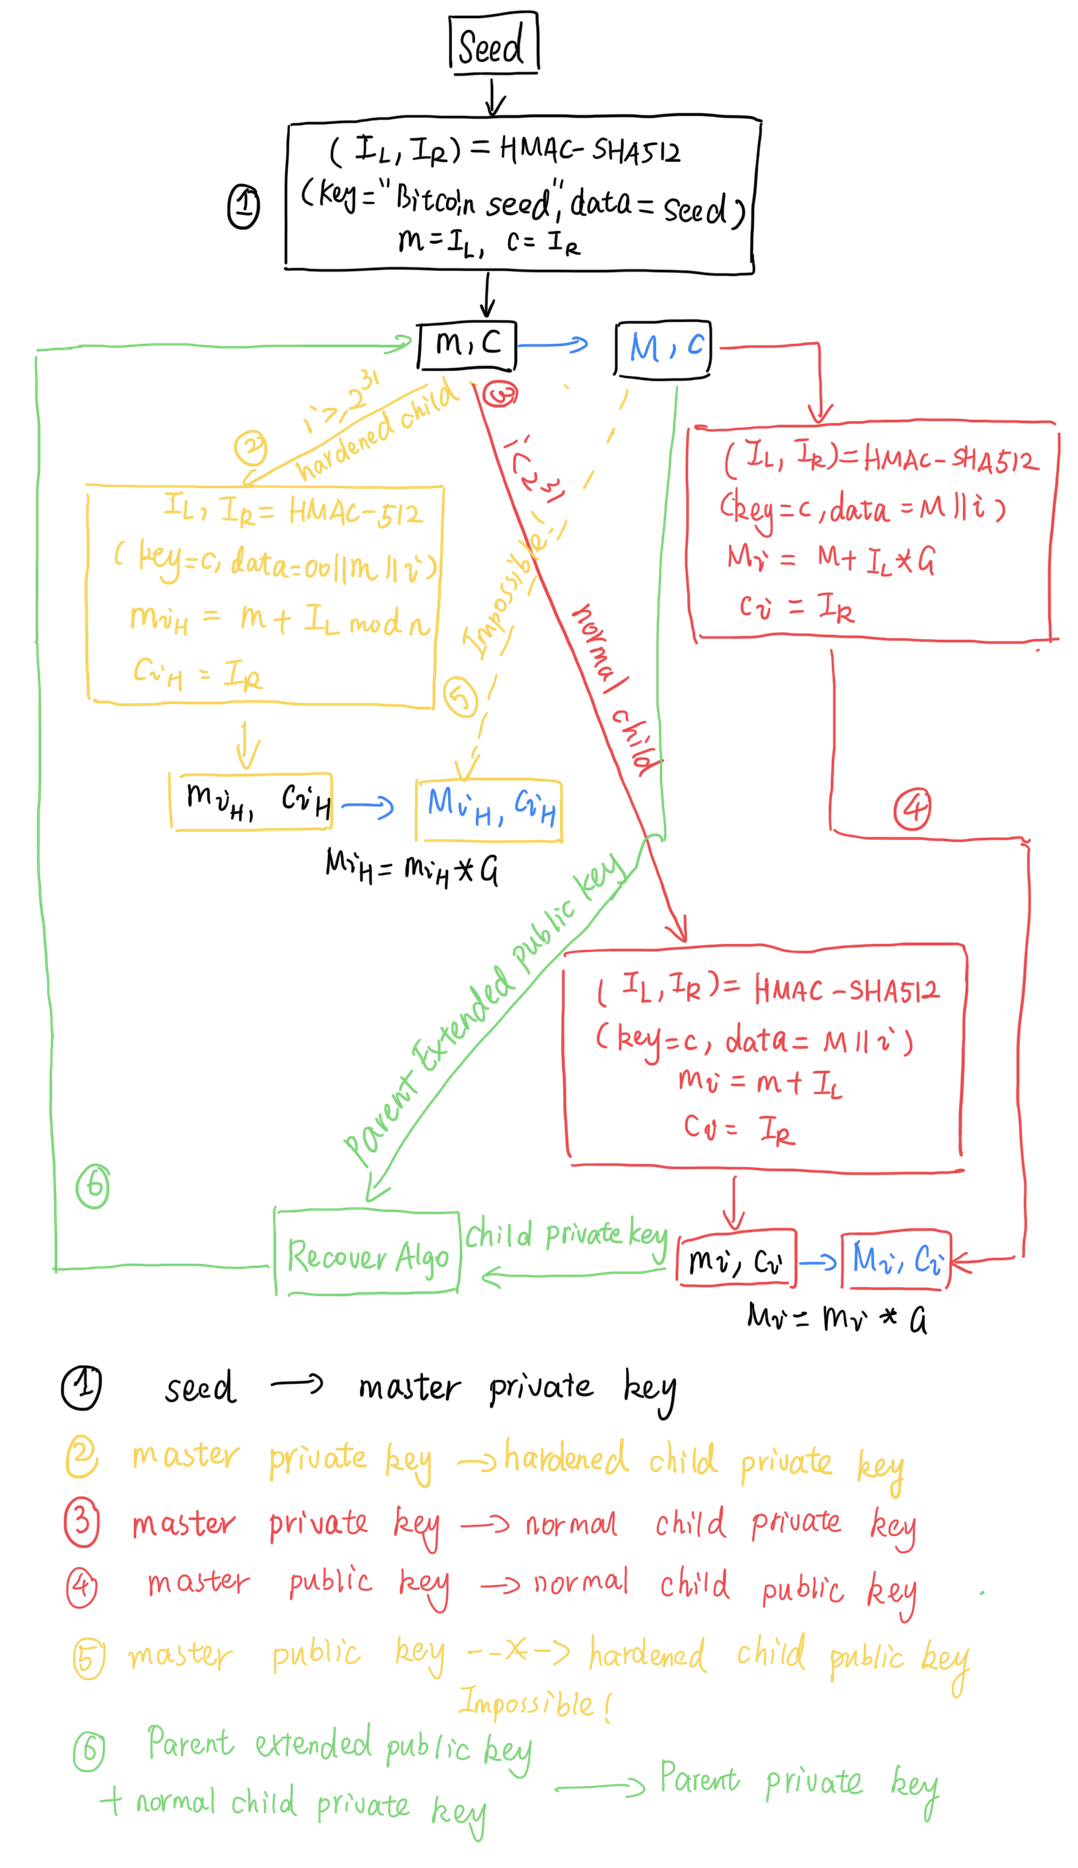
\includegraphics[width=.8\textwidth]{./outline.png}
\caption{密钥树派生图}\label{fig-parsesig}
\end{figure}

\subsection{Logic Hierarchy for Determined Wallets in BIP44}

为了方便标记,将CKDpriv(CKDpriv(CKDpriv(m,$3_H$),2),5) 记为 $m/3_H/2/5$,
将CKDpub(CKDpub(CKDpub(M,3),2),5) 记为 $M/3/2/5$。其中m代表主私钥,M代表主公钥。
BIP44对确定性钱包的逻辑层次做了如下限定:

$$m / purpose' / coin-type' / account' / change / address-index$$
其中,$'$代表了这一层使用的是hardened child的派生方式。

\begin{itemize}
\item Purpose被设定为一个常量$44‘(0x8000002C)$,代表了这棵树的逻辑层级是符合BIP44规范的。
\item Coin type: 对每个不同的数字货币建立了独立的子树空间。对于每种数字货币,
coin type是一个常量,需要开发者为他们的项目申请尚未使用的值。
\item Account: 根据不同的用户身份以及使用目的对密钥空间进行划分,允许钱包将不同账户隔离开来。Account从0 开始递增。在当前账户没有任何交易历史的情况下,钱包软件需要阻止新账户的生成,
并且在用户从外部导入种子(master seed)后,钱包需要恢复所有已经使用过的账户。
\item Change: $`0`$代表外部的密钥链,即需要暴露给其他人用来收款的地址。$`1`$代表内部的密钥链,
对于外部是不可见的,如用作找零地址等。
\item Index: 地址从0开始连续递增,该index即为BIP32中定义的用于派生子节点的child index。
\end{itemize}

\begin{table}
\centering
\caption{Example}
\begin{tabular}{|c|c|c|c|c|}
\hline
\small
Coin &  Account  &   Chain  &  Address &  Path \\\hline
Bitcoin &  first  &  external &  first &  m/44'/0'/0'/0/0 \\\hline
Bitcoin &  first  &  change &  first &  m/44'/0'/0'/1/0 \\\hline
Bitcoin Testnet &  second  &  external &  second &  m/44'/1'/1'/0/1\\\hline
Bitcoin Testnet &  second  &  change &  first &  m/44'/1'/1'/1/0\\\hline
\end{tabular}
\end{table}

\subsubsection{Account Discovery}
用户从外部导入master seed后,钱包需要对用户使用过的账户进行恢复,过程如下:
\begin{itemize}
\item Derive the first account's node (index = 0).
\item Derive the external chain node of this account.
\item Scan addresses of the external chain; respect the gap limit described below.
\item If no transactions are found on the external chain, stop discovery.
\item If there are some transactions, increase the account index and go to step 1.
\end{itemize}
 Gap limit目前被设置为20,即当扫描到某个账户k的external chain里有连续20个没有被使用的地址时,
 钱包就会认为当前的账户还没有被使用,就停止继续扫描。
该算法有效的前提是,存在账户没有被使用时,钱包需要阻止用户通过递增index继续生成下一个新账户,
并且在同一个账户内部,存在20个连续的地址没有被使用时,阻止用户跨越这些地址生成下一个新地址。


\subsection{Security}
\label{sec-security}
\textbf{该方案能够提供的安全性}
\begin{itemize}
\item 给定一个公钥K,攻击者计算出相应私钥k的难度至少和解决椭圆曲线离散对数问题一样难
(这是由基于椭圆曲线的密码学方案所提供的)。
\item 给定一个extended private key$(k_i,c_i)$以及对应的$i$,攻击者恢复parent private key $k_{par}$至少和对HMAC-SHA512进行暴力攻击一样难,即至少需要进行$2^{256}$次HMAC-SHA512计算。
\item 给定任意数量($2\leq N\leq 2^{32}-1$)的(index,extended private key)对($i_j,(k_j,c_j)$),
确定他们是否是由同一个parent extended private key 派生出来的,至少和对HMAC-SHA512进行暴力攻击一样难,
即至少需要进行$2^{256}$次HMAC-SHA512计算。
\end{itemize}

\textbf{以下两种场景是不安全的}
\begin{itemize}
\item 给定一个parent extended public key$(K_{par},c_{par})$ 和一个normal child public key $(K_i)$,
找到该child对应的i是容易的。\\
对于normal child,i的取值范围为$0~2^{31}-1$,给定上述条件,
可以通过遍历i来重复child public key 派生的过程,并比较派生出的public key是否与给定的child public key相等,如相等,则对应i就是该child对应的index。

\item 给定一个parent extended public key $(K_{par},c_{par})$, 
和normal child private key $(k_i)$, 找到$k_{par}$是容易的。\\
根据前一部分的推导,可以计算出该child对应的index i。  
由于I = HMAC-SHA512(Key = $c_{par}$, Data = $ser_P$($K_{par}$) || $ser_{32}$(i))=($I_L,I_R)$, 
而 $k_i$=($parse_{256}(I_L)$) + $k_{par}$ $(mod$ $n)$.   
因此 $k_{par}$=$k_i-$($parse_{256}(I_L)$)$(mod$ $n)$
\end{itemize}    

第二条性质对于安全性的影响比较关键。这意味着知道一个parent extended public key 
以及 private non-hardened child key
即意味着知道了parent extended private key,因此对待extended public key 
应该比普通的public key 更加小心。
而对于hardened 节点,因为它们只能由parent extended private key来派生,
所以安全性相对较好一些(不存在上述问题),这也是在BIP44中规定在
purpose, cointype, account层使用hardened 节点的原因(防止这三层上一层的私钥被攻击者按上述过程恢复出来)。


\subsubsection{Implementation}
当知道了parent extended public key 以及 child private key后,
parent private key的恢复过程如下:
(以下代码基于一个BIP32钱包的Python库bip32utils\footnote{\url{https://github.com/lyndsysimon/bip32utils}})

\begin{lstlisting}[language=python,label=lst-recover]
CURVE_GEN  = ecdsa.ecdsa.generator_secp256k1
CURVE_ORDER  = CURVE_GEN.order()
BIP32_HARDEN = 0x80000000 
def recover_parent_privkey(parent_pubkey,child_privkey):
	# traverse all possible non-hardened child index (0~2^31-1) to 
	find the corresponding index of child_privkey
	for i in xrange(0, BIP32_HARDEN +1):
		child=parent_pubkey.CKDpub(i)
		if(child.PublicKey()==child_privkey.PublicKey()):
			break
    # if i is larger than 2^31-1, means that it corresponds to a hardened child, 
    then the recovery is impossible
	if i & BIP32_HARDEN:
		print "can not recover parent private key with a hardened child node"
		return
	# data is composed of public key || i
	data=parent_pubkey.PublicKey()+struct.pack(">L",i)
	(Il,Ir)=parent_pubkey.hmac(data)
	Il_int = string_to_int(Il)
	if Il_int > CURVE_ORDER:
	    return None
	cpk_int=string_to_int(child_privkey.k.to_string())
	# recover parent private key ppk_int from cpk_int= ppk_int + Il_int mod n
	ppk_int=(cpk_int-Il_int)%CURVE_ORDER
	return int_to_string(ppk_int).encode('hex')
\end{lstlisting}


